% Controlling a tensegrity robot brings multiple challenges such as distributed controls, nonlinear interactions between components and handling difficult to model dynamics such as oscillations. 
% % For this reason traditional centralized controllers and centralized designs are not a good match for a tensegrity robot. 
% In contrast WE present a decidedly distributed approach for controlling a tensegrity robot. 
% On the hardware side, the core of OUR design is an independently controllable rod containing two independent ``end-cap'' controllers on each side of the rod. This model naturally matches the distributed yet holistic nature of a tensegrity. The controllers act independently of each other but they interact through the system, where changing lengths of one of the MUSCLES affects the whole structure in a non-linear way. This behavior can be seen in Figure
% \ref{fig:nonlinear}. When WE pull only one of the MUSCLES (muscle 13), all the MUSCLES change their length while some of them get shorter and some of them get longer. 

% \begin{figure}[t]
% \centering
% 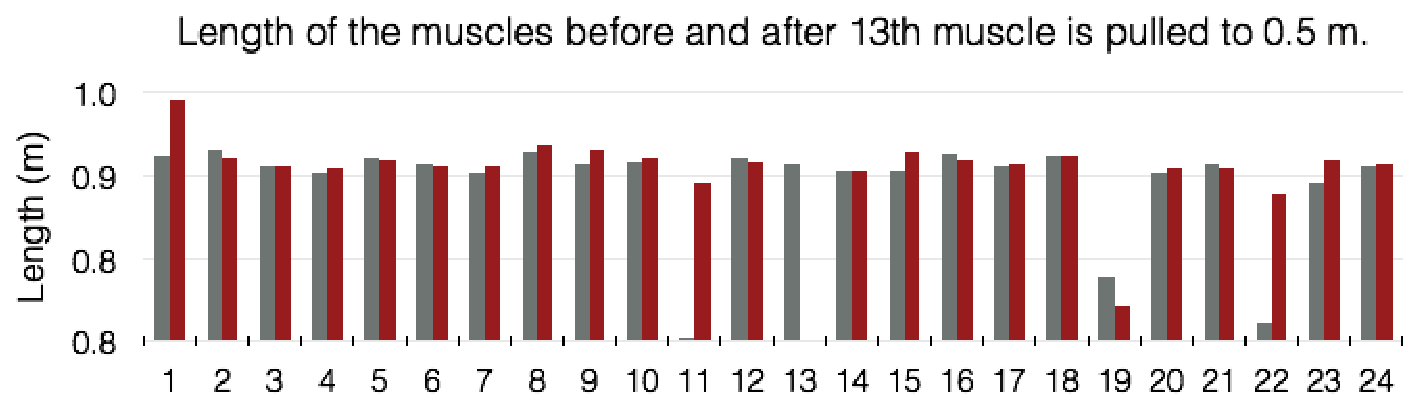
\includegraphics[width=\columnwidth]{tex/ASME-journal/results/actuate1/actuate1.eps}
% \caption{Change in length of the MUSCLES when one of them (13th) is pulled to 0.5 meters while other MUSCLES keep the same rest length as before.  Grey bars show original length, red show final length. While the robot is at the exact same orientation, the actual lengths of the MUSCLES change in a non-linear way.  Some of the MUSCLES shorten due to the tension introduced by muscle 13, some of the MUSCLES relax.}
% \label{fig:nonlinear}
% \end{figure}

% To facilitate distributed assembly, the controllers communicate via wifi wireless network. This design allows for simplified construction, and reduces cabling problems that could arise if the tensegrity robot needs to roll through adverse conditions. This design is not only distributed, but modular. For a simple six-bar tensegrity, WE can simply assemble six identical rods to form the tensegrity robot. In addition for more complex designs additional rods can be used without changing the design of the rods themselves.

% OUR next challenge is to control a set of assembled rods into a high-performance tensegrity robot. To do this, WE need controls that are able to work in a distributed control environment, and also work when wireless communication may not be high-bandwidth or reliable. To overcome this problem, WE use distributed controls and distributed learning, where each controller learns its policy, but the overall behavior requires coordination of these controllers to make the tensegrity robot move. The setup described is a coordination learning problem where WE have independent learners working towards a shared goal. 
% % The details of the learning distributed controls for this setup is described at the Section \ref{sec:learning}.

% An additional control challenge is how to handle the physical hardware limitations of each actuation system. Ideally WE would like OUR controller to be able to simply dictate the actual lengths of each muscle it is responsible for. However, due to the overall tension caused by the rest of the structure, the controllers can only provide the rest length of the muscles.  Since the MUSCLES are flexible, the actual lengths change out of the control of the controller. 

% In addition, the hardware limitations also play an important role when tensions get higher. Since all the motors in the robot pull against each other, it is possible to reach tensions that the motors cannot handle. Moreover, since the rest of the structure can potentially overpower any one motor, there  is a chance that a motor is back-driven and forced to feed out some of the cable stored on the spool. To address these limitations, if the muscle is experiencing tensions above the motor limit, and the cable is pulled to its maximum length of 1.1 meters, the simulation is stopped and the policy is considered as not feasible.

% To stay within the bounds of the physical hardware, WE simulate the motors with high level controllers that has constant speed (0.2 m/s) while the tensions stay within reasonable limits. Indeed, the physical motors on the SUPERBall can pull with 0.5 m/s within the tension range that WE are dealing with, but WE selected 0.2 m/s in order to leave plenty of hardware headroom and also to lower power consumption. While the motors move with constant velocity, the controllers dictate preferred positions for the motors. Dictating preferred position is exactly same as dictating preferred rest length if the cables do not slip. Every timestep, the motors pull or release their cables with constant speed to get closer to their goal. While staying in reasonable tensions, this setup is feasible on the real robot. The assumption is that there is an intermediate controller layer that regulates the voltage vs torque to provide constant speed rotation.

The overall goal of this controller is to have the tensegrity robot roll smoothly within the limitations of the simulated actuation and hardware parameters. 
A periodic open loop controller is used with parameters that are set by an evolutionary algorithm~\cite{back1997handbook}. 
During rolling locomotion, the controllers will repeat the same actuation motion. 
Considering that the rolling locomotion is a repetitive behavior, the signals produced by the controllers will be periodic. 
The key to making this system work is determining the shape of this periodic signal.

For this work, a signal of periodicity \(t\) has a function \(F(t)\) where the function is a discrete number of step functions \(n\).
Thus, a simplistic example where \(n = 2\) would have the form

\begin{align}
F(t') =
  \begin{cases}
    y1       & \quad \text{for} t' \in [0, t_{1}]\\
    y2       & \quad \text{for} t' \in (t_{1}, t]\\
  \end{cases}
\end{align}

where \(t_{1} < t\) and \(y1\) and \(y2\) are motor position values and this simple case can be seen in figure~\ref{fig:signal}.

\begin{figure}[t]
\centering
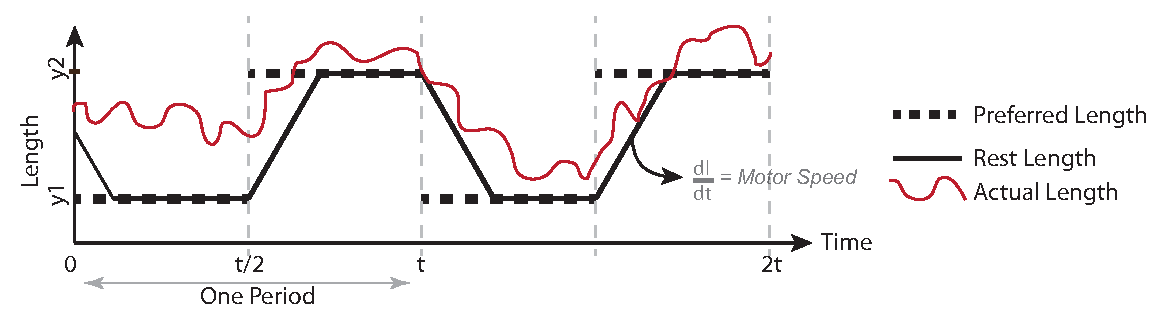
\includegraphics[width=\columnwidth]{tex/ASME-journal/fig/signal.eps}
\caption{An example signal with 2 sub-intervals with preferred lengths of y1 and y2 and periodicity t.}
\label{fig:signal}
\end{figure}

When the function is expanded to \(n = k\) it takes the form of

\begin{align}
F(t') =
  \begin{cases}
    y1       & \quad \text{for} t' \in [0, t_{1}]\\
    y2       & \quad \text{for} t' \in (t_{1}, t_{2}]\\
    \vdots   & \quad \vdots \\
    yk       & \quad \text{for} t' \in (t_{k-1}, t]\\
  \end{cases}
\end{align}

and it can easily be shown that as \(n \to \infty\) any arbitrary signal may be generated.
To generate a signal, the only parameters needed are number of sub-intervals and rest length values for each sub interval. 
For the specific example given in Figure \ref{fig:signal}, the number of subintervals is 2 and y1 and y2 are the values of preferred rest lengths for those intervals. 

% Let's assume that the periodicity of the signal is $t$ and WE represent the signal as $F(x)$ , $x$ being time within interval $[0,t]$. There are many possible ways to represent this control function. For instance a natural choice would be a sine wave, or a series of overlapping waves to form more complex control policies. To reduce complexity, in this paper WE use an even simpler control model: WE break down each control interval into sub-intervals and assign different preferred rest lengths for each sub-interval.  Considering the limited velocity of the motors, the motor will slowly move to reach these selected points during those sub-intervals. The control model is essentially a set of overlapping square waves. As an example, WE can divide one period to 2 sub-intervals, where the motor will have a preferred length of $y1$ for the first half of the signal, and $y2$ for the second half of the signal. With the motor moving towards $y1$ and $y2$, the resulting signal will be similar to the Figure \ref{fig:signal}. 


% To generate a signal, the only parameters needed are number of sub-intervals and rest length values for each sub interval. 
% For the specific example given in Figure \ref{fig:signal}, the number of subintervals is 2 and y1 and y2 are the values of preferred rest lengths for those intervals. 
% The example given in the Figure \ref{fig:signal} is a simple signal, and while number of sub-intervals is low, the complexity of the signals that can be generated is limited. 
% On the other hand, the complexity of the possible signals increases with the number of sub-intervals. 
% Due to this, from now on, WE will refer to this parameter as the complexity degree  ($n$) of the signal. 
% Depending on the complexity degree and the values of $y_1,y_2,...y_n$, the shape of the signal can change between typical trapezoid, zigzags, stairs or combination of those. 

% To summarize, the complexity of the signal depends on $n$ and each controller has $n$ number of inputs depending on the complexity selected. The rest lengths of the signal follows this signal, and actual lengths of the MUSCLES change according to other MUSCLES and interaction of the robot with the environment. Each controller has a separate signal and it controls only one of the motors. 24 motors controls 24 MUSCLES independently but affecting each other with the common goal of rolling locomotion.


% While the control parameters  to generate the signal are straightforward, the interaction between these signals to reach a rolling behavior is highly complex. As explained before, the  nonlinear and oscilattory nature of the problem makes the tensegrity hard to control with classical control methods. The consequences of specific signal combinations can be simulated, but finding the correct signal parameters for a specific behavior is not possible. In this section WE explore how WE can use the simulation combined with a fitness evaluation to implement an evolutionary algorithm that can evolve a set of control parameters that leads to the desired behavior.

% Evolutionary algorithms are a family of biologically inspired learning methods, where new candidate solutions for a problem are generated, evaluated and eliminated repeatedly \cite{back1997handbook}. Evolutionary algorithms consists of the cycle of  forming new members, assigning fitness and selecting the most fit members. This cycle is called a generation and it is repeated until desired behavior is obtained. 

\subsubsection{Algorithm and Learning Method}
The problem is episodic, the agents have 60 seconds to test their policies. At the end of each episode these candidates are evaluated according to their performance. 
Performance is then measured as the distance covered in 60 seconds. 
Formally, the evaluation is defined as

\begin{equation}
\label{eq:r}
f = d(y_{0,0},y_{0,1},...,y_{0,n},y_{1,0},...,y_{24,n}) \;,
\end{equation}

where, $y_{i,j}$ is the rest length for the $i$th controller and $j$th subinterval. 
Depending on the complexity of the signals ($n$) selected, there are $24 * n$ parameters to learn. 
% For this study, WE used the historical average method that WE previously developed and tested with earlier versions of NTRT to obtain rolling behavior using sine wave signals (REF). 
In order to learn these parameters, this method uses a historical average co-evolutionary algorithm.
In historical average, each member receives its fitness according to the average of their performances.
If a member survives for the next generation (is not eliminated or mutated) the member keeps  its previous experiences. 
At each generation, the fitness assignment is the average of this growing history of past evaluations. 
% The overall cooperative coevolutionary algorithm with historical average fitness assignment can be found in Algorithm \ref{Alg:CCEA-AA}.
The algorithm used can be found in Algorithm~\ref{Alg:CCEA-AA}.

% Note that the decomposition of the distance function $d$ is not readily obtainable in closed form. Instead it must be computed from observing simulations or measured from a physical implementation. Also note that OUR evaluation does not explicitly take any behavior into account besides the distance moved (final position - initial position). Tensegrities can exhibit many different gaits, ranging from hopping to rolling, and many different paths, ranging from spirals to straight lines. However, tensegrities that maximize final vs initial position tend to roll towards one direction. Deviations from this pattern tend to hurt performance.


\begin{algorithm}[th]
 \SetAlgoLined
 \KwData{Population of $n$ elements for each agent}
 \For{i=1..$k$}{
  $random_{team} \leftarrow \emptyset$ \;
  \ForAll{Populations} 
  {
  	$random_{team} \leftarrow random_{agent}$\;
  }
  score = evaluate($random_{team}$) \;
  \ForAll { agents $\in$ $random_{team}$}
  {
  	agent.history $\leftarrow$ score \;
%  	\If{score $>$ agent.score}
%  	{
%  		agent.score $=$ score \;
%  	}
  }
  }
 \ForAll{ Populations }
 {
   \ForAll { agents}
   {
   	   agent.fitness $= \text{average}$(agent.history) \;
   }
 	order population according to the fitness\;
 	eliminate the last $z$ members\;
 	copy the first $z$ to the last $z$\;
 	mutate the last $z$\;
 	clear history for the last $z$\;
 }
 
\caption{Cooperative coevolutionary Algorithm with Historical Average}
\label{Alg:CCEA-AA}
\end{algorithm}

% The problem that WE are working on is distributed by nature. The controllers are independent and there is not a centralized mechanism. To work on such problems, cooperative coevolutionary algorithms (CCEA) is a class of algorithms that extends evolutionary algorithms. Instead of one particular solution for the problem, there are multiple agents. Multiple agents have to coordinate to solve a problem or to optimize an outcome \cite{wiegand2003analysis}. Each agent has a separate population that evolves independently. On the other hand, to evaluate the members of these separate populations, the agents have to form a team for fitness assignment, because the task needs cooperation of the agents to maximize the rolling behavior. At each experiment 1 member from each population are chosen randomly to form a team. This set of policies form the team for that experiment. In OUR problem, WE have 24 agents which means 24 populations.

% Each agent optimizes $n$ parameters while they are judged based on their performances within different teams formed during evaluation phase. At each evaluation phase, each member is evaluated multiple times. To move on to the elimination phase, each member has to be assigned a single fitness number using these values. The literature contains multiple approaches to this problem such as taking the maximum score (leniency), testing each member with best team so far (hall of fame) or average score \cite{wiegand2003analysis,panait2008theoretical,Iscen:2013aa}.

% For this study, WE used the historical average method that WE previously developed and tested with earlier versions of NTRT to obtain rolling behavior using sine wave signals (REF). In historical average, each member receives its fitness according to the average of their performances, moreover, if a member survives for the next generation (is not eliminated or mutated) the member keeps  its previous experiences. At each generation, the fitness assignment is the average of this growing history of past evaluations. The overall cooperative coevolutionary algorithm with historical average fitness assignment can be found in Algorithm \ref{Alg:CCEA-AA}.


\subsubsection{Learning Results}
An example learning session is shown using signals with complexity ($n$) of 5 and period ($t$) of 4 seconds.  
Figure \ref{fig:learning} illustrates the distance rolled by the robots over the course of learning. 
Starting with 0 meters, the robots converge to rolling over 32 meters in 60 seconds. 
This result shows that successful learning of rolling locomotion using CCEA is possible. 
% In Section \ref{sec:platform} WE discussed when a policy is labeled as unfeasible during learning.  
The second line at the same Figure (Figure \ref{fig:learning}) shows the rate of unfeasible policies that are tried while learning to roll. 
While converging to rolling locomotion, unfeasible policies drop to 0. 
This shows that the learned policy lies within simulated parameters set by the user.

\begin{figure}[t]
\centering
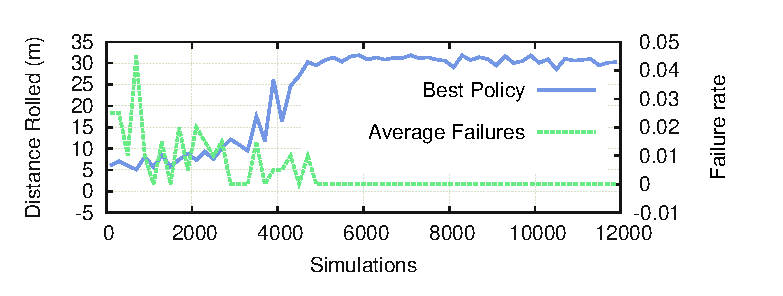
\includegraphics[width=\columnwidth]{tex/ASME-journal/results/failures/learningVsFailures.eps}
\caption{The performance of the robots during the learning session for signals of complexity 5 and period of 4 seconds. As a side result, the percentage of the policies that were failed to stay in reasonable limits are shown with the second line. }
\label{fig:learning}
\end{figure}

% Considering that the robot has a shape that is similar to a sphere with a diameter of 1.5 meters, rolling 32 meters  means  approximately 7 revolutions in a minute. 
% This results in 8 seconds per revolution. 
% Considering that WE selected 4 seconds as periodicity of the signal, the learned signals  provide half revolution, and applying same signals also results in the other half of the one complete revolution.  
% This supports the reasoning behind selecting periodic signals to obtain rolling locomotion as a periodic movement of the robot.

% \begin{figure}[t]
% \centering
% 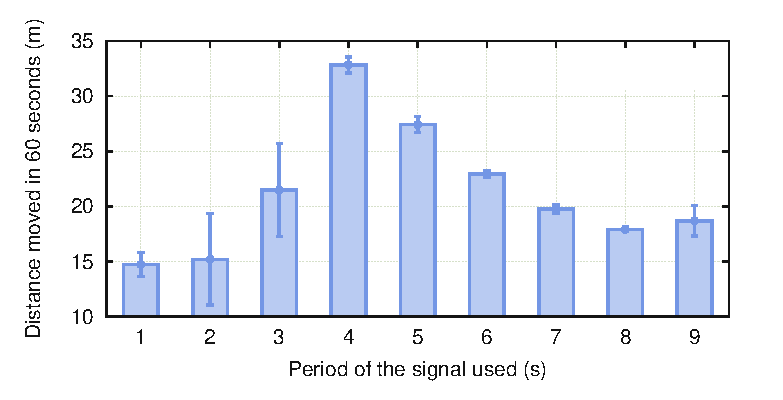
\includegraphics[width=\columnwidth]{tex/ASME-journal/results/period/period.eps}
% \caption{The performance of the converged policies after learning for signals with periods of different lengths, while the complexity is fixed to 5 points. The best performance is reached with signals that are repeated every 4 seconds. Signals with longer periods have a decreasing performance proportional to the inverse of the periodicity.}
% \label{fig:period}
% \end{figure}


% \begin{figure}[t]
% \centering
% 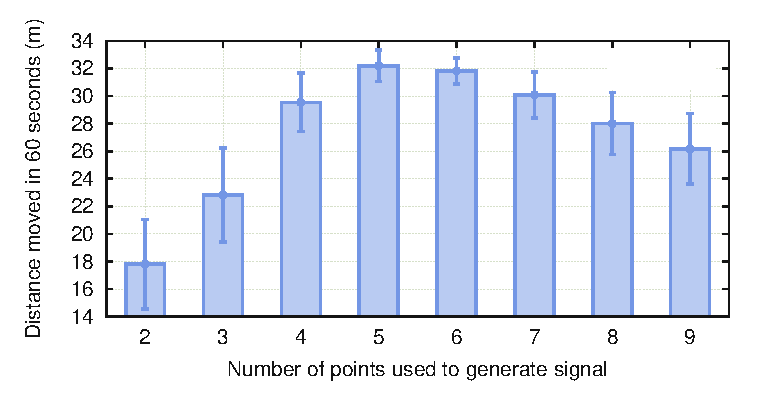
\includegraphics[width=\columnwidth]{tex/ASME-journal/results/complexity/complexity.eps}
% \caption{The performance of the converged policies after learning for signals with different complexity levels, while the periodicity is fixed to 4 seconds. The best performance is reached with signals that use 5 points. Less complex signals cannot generate rolling locomotion, and more complex signals are hard to learn.}
% \label{fig:complexity}
% \end{figure}

% % The first set of experiments illustrated when $n$ and $t$ are selected as 5 and 4 (4 seconds with complexity of 5). Next, WE investigate the results of learning using signals with different complexity and periodicity. Figure \ref{fig:period} shows the converged behaviors when WE fix  $n$ to 5 and learn using variable $t$. Note that the signal used for different values of $t$ is not the same. The signals are learned from scratch for each value of $t$. 

% % Clearly, the peak is when the signals have periods of 4 seconds (frequency of 0.25 Hz). When WE shorten the period below 4 seconds, the robot cannot learn to roll. One can think that providing the same signal with a higher frequency can provide the same rolling behavior, but when the tensegrity deforms to start rolling with a higher speed, the contact forces from the ground and the reaction of the structure changes completely. When WE increase the periodicity to longer than 4 seconds, the frequency drops and the performance gradually decreases as expected. Moreover,  the rolled distance is linearly proportional to the frequency. For the values of $4$ to $8$ seconds, the performance divided by the frequency give the same value ($\frac{33}{1/4} \simeq \frac{27}{1/5} \simeq \frac{22.5}{1/6} \simeq \frac{19}{1/7} \simeq 132 $). 


% Next, WE investigate the effects of different signal complexity level to the learning.  The period is fixed at 4 seconds, because it gave the best score combined with the complexity of 5 in previous set of experiments (Figure \ref{fig:period}). WE started with the complexity of 2, where the signal is simplest possible. It alters between one high value for the first 2 seconds, and one low value for the last 2 seconds. WE increase the complexity up to 9 points. The result is illustrated at Figure \ref{fig:complexity}.  The first conclusion is that signals with complexity 2 cannot succeed at learning to roll, but the performance increases with higher complexity. Clearly the controllers need more complex signals to provide rolling locomotion. The peak performance is reached at complexity 5, where the preferred length alters between 5 different points during 5 intervals of 0.8 seconds each. 

% The second conclusion of this experiment is seen when the complexity increases even further.  The learned behavior gradually decreases and error bars show that statistical significance goes down. The reason behind this behavior is that the parameters to learn increase linearly, and the problem to learn becomes linearly harder for each controller. Since all the controllers learn simultaneously while interacting with each other, overall hardness of the problem is increased even further. The error bars show that in more complex problems, some statistical tests reach good results while some of them fail completely due to the hardness of the problem.

% \subsection{Analyzing the Rolling Behavior}
% \label{sec:openResults}

% In previous section, WE showed that learning to roll for a tensegrity robot succeeds with signals of right periodicity and complexity. In this section, WE look at the learned behavior and analyze 
% the feasibility of the behavior, lengths and tensions during rolling, converged signals and robustness of the behavior.

% As a sample learning behavior, WE select one of the learned behaviors with periods of 4 seconds and complexity of 5. The learning process for this behavior was illustrated in Section \ref{sec:learning} and Figure \ref{fig:learning}. For each simulation, the robot tests different policies for 60 seconds, and the distance moved is marked as the score. The policies that are tested are updated according to the Cooperative Coevolutionary Algorithm with Historical Average (Algorithm \ref{Alg:CCEA-AA}). For this particular experiment, the robots reach the performance of rolling 32 meters around 5000 simulation steps. As a side result, the percentage of failed policies (due to high tension) reaches 0.

% \begin{figure}[t]
% \centering
% 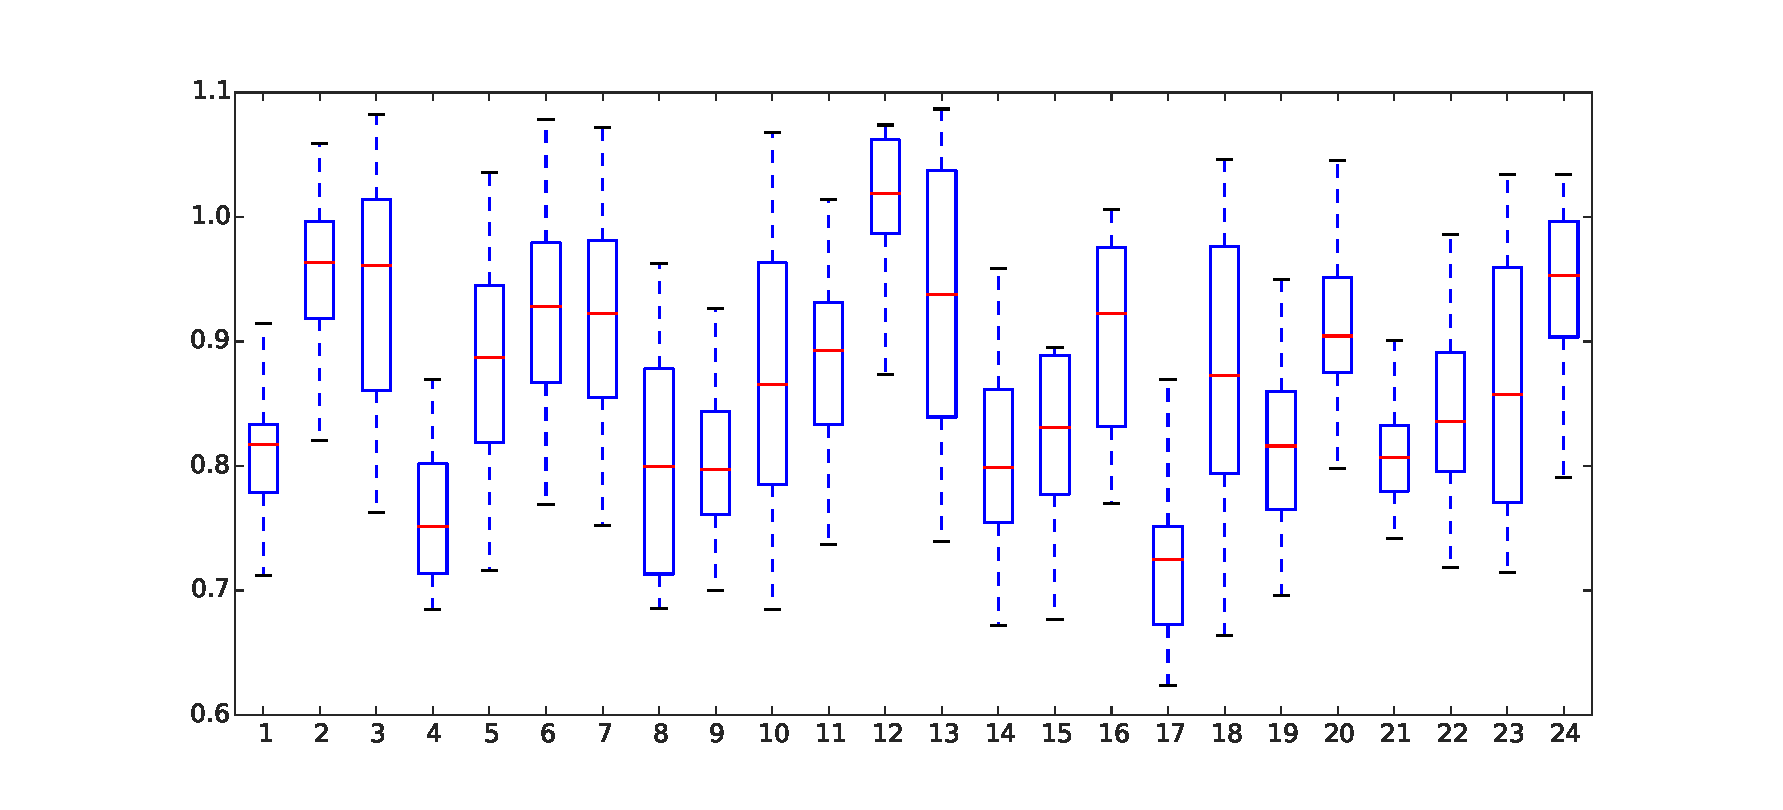
\includegraphics[width=\columnwidth]{tex/ASME-journal/results/signals/policy.eps}
% \caption{A sample learned policy for 24 motors is illustrated. For each signal, the red line at the center shows the mean of the signal and the box and the dashed lines show the interval that the signal lies in.}
% \label{fig:policy}
% \end{figure}

% First, WE take this learned behavior and look at the learned policy. Figure \ref{fig:policy} shows the intervals that each muscle's length lies within.  The muscles' lengths vary from 0.7 m to 1.1 m. While some of the MUSCLES such as 1 and 21 have minimal change in length, some of them (such as 13 and 23) changes bigger intervals. Another remark is that, the mean of the signal (that is noted by the red horizontal line) is not necessarily at the center of the interval that the signal lies in. This is one difference that more complex signals provide. For example, the length of the muscle number 1 is mostly around 0.82 m, but it reaches as low as 0.7 once in a while.
 
% \begin{figure}[th]
%         \centering
%         \begin{subfigure}[b]{0.9\columnwidth}
%                 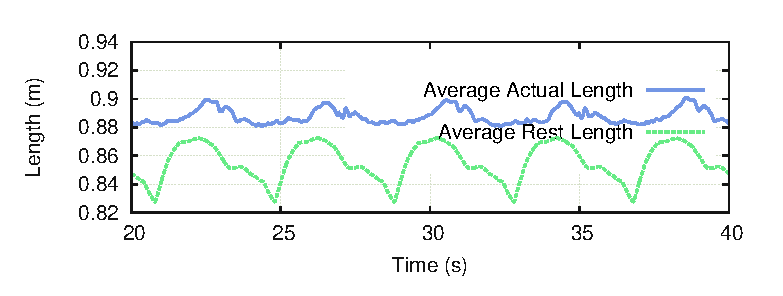
\includegraphics[width=\textwidth]{tex/ASME-journal/results/tension-energy/lengths.eps}
%                 \caption{Average Rest Lengths and Actual Lengths of The Muscles}
% 				\label{fig:lengths}
%         \end{subfigure}\\
%         \begin{subfigure}[b]{0.9\columnwidth}
% 				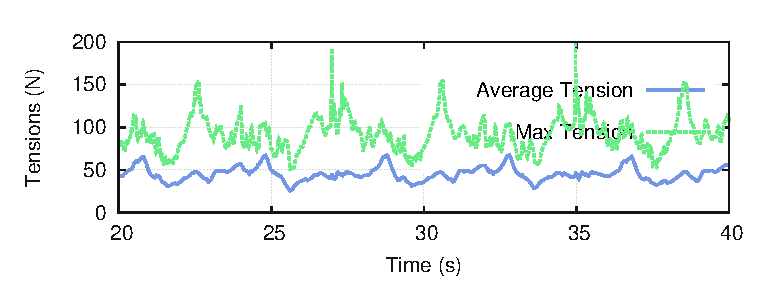
\includegraphics[width=\textwidth]{tex/ASME-journal/results/tension-energy/tensions.eps}
%                 \caption{Average and Maximum Tensions of the Muscles}
% 				\label{fig:tensions}
%         \end{subfigure}\\
%         \begin{subfigure}[b]{0.9\columnwidth}
%                 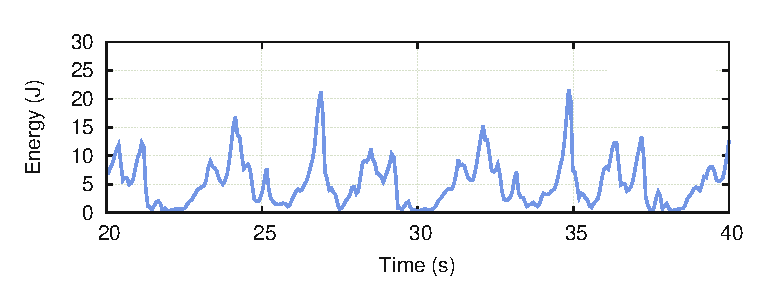
\includegraphics[width=\textwidth]{tex/ASME-journal/results/tension-energy/tensKinEnergy.eps}
%                 \caption{Kinetic Energy of the Tensegrity Robot}
%                 \label{fig:KinEnergy}
%         \end{subfigure}\\
%          \begin{subfigure}[b]{0.9\columnwidth}
%          		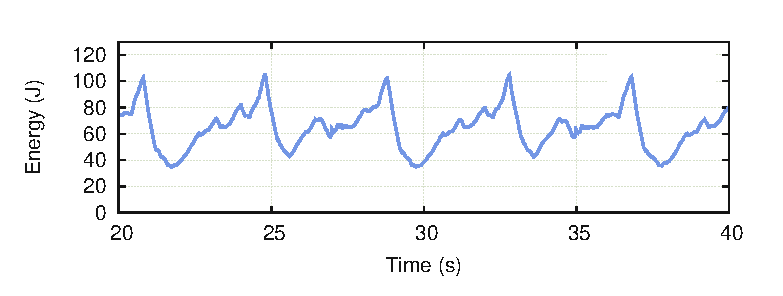
\includegraphics[width=\textwidth]{tex/ASME-journal/results/tension-energy/tensPotEnergy.eps}
%                 \caption{Total Potential Energy Stored in Muscles}
%                 \label{fig:PotEnergy}
%         \end{subfigure}
%         \begin{subfigure}[b]{0.9\columnwidth}
%          		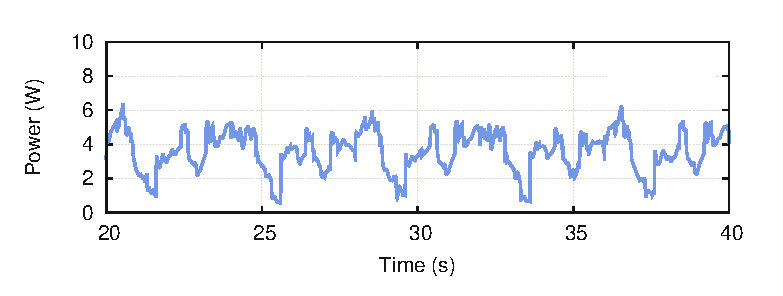
\includegraphics[width=\textwidth]{tex/ASME-journal/results/tension-energy/power.eps}
%                 \caption{Power Used by the Motors to Roll}
%                 \label{fig:power}
%         \end{subfigure}
%         \caption{Illustration of different aspects of the Tensegrity Robot over time, during rolling locomotion. The used signals for MUSCLES repeat themselves every 4 seconds. The tensegrity robot completes one revolution in 8 seconds. Tensions, Lengths and Power usage of the robot stays in OUR defined limits for the hardware. }
%         \label{fig:RollingAnalyze}
% \end{figure}


% One way to analyze rolling behavior is looking at the average lengths and tensions of the MUSCLES in addition to the potential and kinetic energy of the structure. First, WE look at how the actual lengths of the MUSCLES change compared to the signals provided. Figure \ref{fig:lengths} shows the average rest length of the MUSCLES (signal provided) and the average actual length of the muscles. The area between the two lines shows the stretch of the MUSCLES due to the tension. The most interesting fact about this graph is the difference of frequencies for the two lines. Although the signals that are provided to the MUSCLES repeat themselves every 4 seconds, the actual lengths repeat themselves every 8 seconds. This supports OUR previous conclusion about using signals that have periodicity of 4 seconds can conclude in revolutions that take 8 seconds. The first half of the roll and second half of the roll use same signal, but the ground interactions make the actual lengths differ.



% During the rolling, the average and maximum tensions of the MUSCLES are illustrated in Figure \ref{fig:tensions}. The average tension is low, stays around 60 N. The second line shows the 
% the tension of the muscle with longest stretch at each particular time of the simulation. The value goes up to 200N staying in values that OUR hardware design can handle. The maximum tension graph also repeats itself every 8 seconds as expected.

% When WE observed  the gait learned using OUR simulator, WE see the rolling locomotion does not have a constant speed. Instead, it slows down and speeds up periodically during each revolution. To illustrate this behavior, WE look at the total kinetic energy of all the rods over time in Figure \ref{fig:KinEnergy}. If WE take the interval between two peak points (when t=27 and t=35), the kinetic energy stays at zero for 1 second around t=30s. Moreover, the repetitive acceleration and deceleration can be clearly seen. This behavior creates an inefficiency in terms of energy for the gait. There are two main reasons for this behavior: First, the learning algorithm only optimizes the distance rolled, not the energy spent during motion. Optimizing more than one criteria  is actually part of OUR future work. Second, in this work, WE are testing open loop controllers. Using some feedback from the robot (such as lengths, tensions or orientation) having a smoother rolling experience can be possible. This is also another future work that WE explain in Section \ref{sec:conclusion}.

% Next, WE observe the potential energy stored in the muscles. Figure \ref{fig:PotEnergy} shows the pattern that repeats itself every 8 seconds as expected. First 4 seconds and second 4 seconds are similar but they slightly differ due to different environment reaction during the second half of a complete roll. The pattern shows an overall behavior of increasing the potential energy slowly over time, and releasing it. This matches the kinetic energy behavior that WE observed in Figure \ref{fig:KinEnergy}. The kinetic energy of the structure increases during the few seconds following the moment potential energy is released (i.e. t=25s).

% The last set of experiments analyzes the approximated power usage by the motors during the rolling locomotion. In simulation, the power consumption is approximated using the current tension of the element  and the constant speed that the motors shortens the muscles. As WE explained earlier, the learned behavior is not optimized to be power efficient for this study. On the other hand, WE want to make sure that it is within limits of motors and batteries that will be used in the hardware. Figure \ref{fig:power} illustrates the average power consumption of the MUSCLES that varies between 2 to 6 W per muscle. Considering that the motors always pull against the tension (and all the MUSCLES are  tight all the time) this value is considerably low. Moreover, it is always possible to lower this value by using a feedback controller in future work.


% \section{Analyzing the Roles of Different Muscles}
% \label{sec:signals}



% \begin{figure}
%         \centering
%         \begin{subfigure}[b]{\columnwidth}
%         		\centering
%                 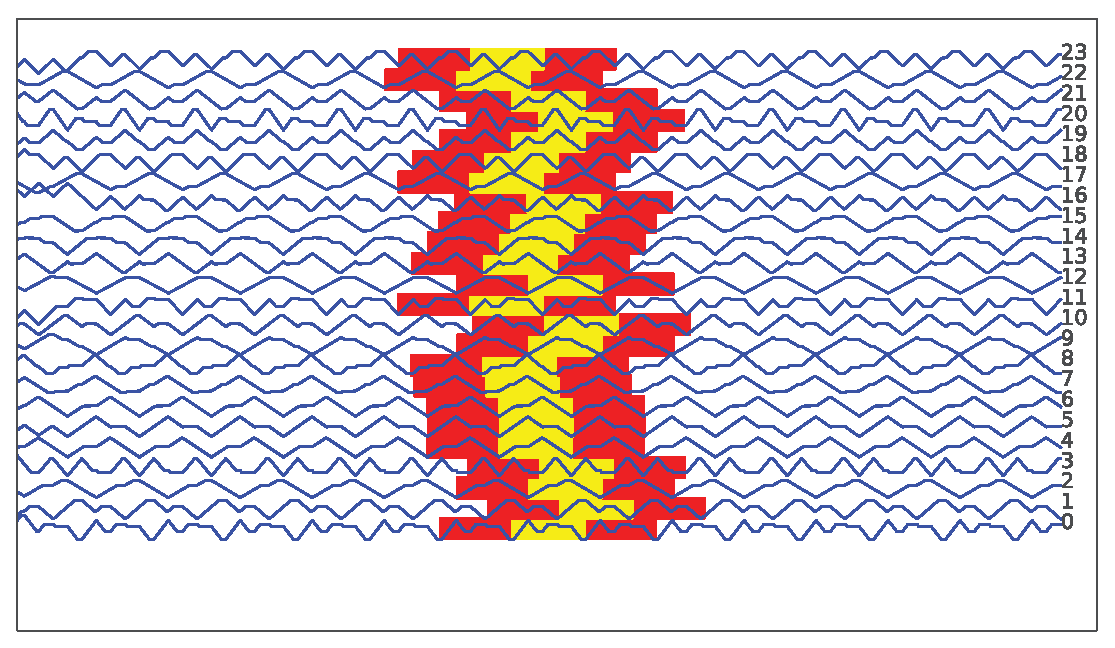
\includegraphics[width=0.7\textwidth]{tex/ASME-journal/results/signals/aligned1.eps}
%                 \caption{The signals of the 24 MUSCLES normalized between [$i$,$i$+1] for muscle $i$. After correlation using time offsets, the highest correlated intervals of 4 seconds are  marked with red,yellow,red pattern. }
% 				\label{fig:aligned1}
%         \end{subfigure}\\
%          \begin{subfigure}[b]{\columnwidth}
%         		\centering
%                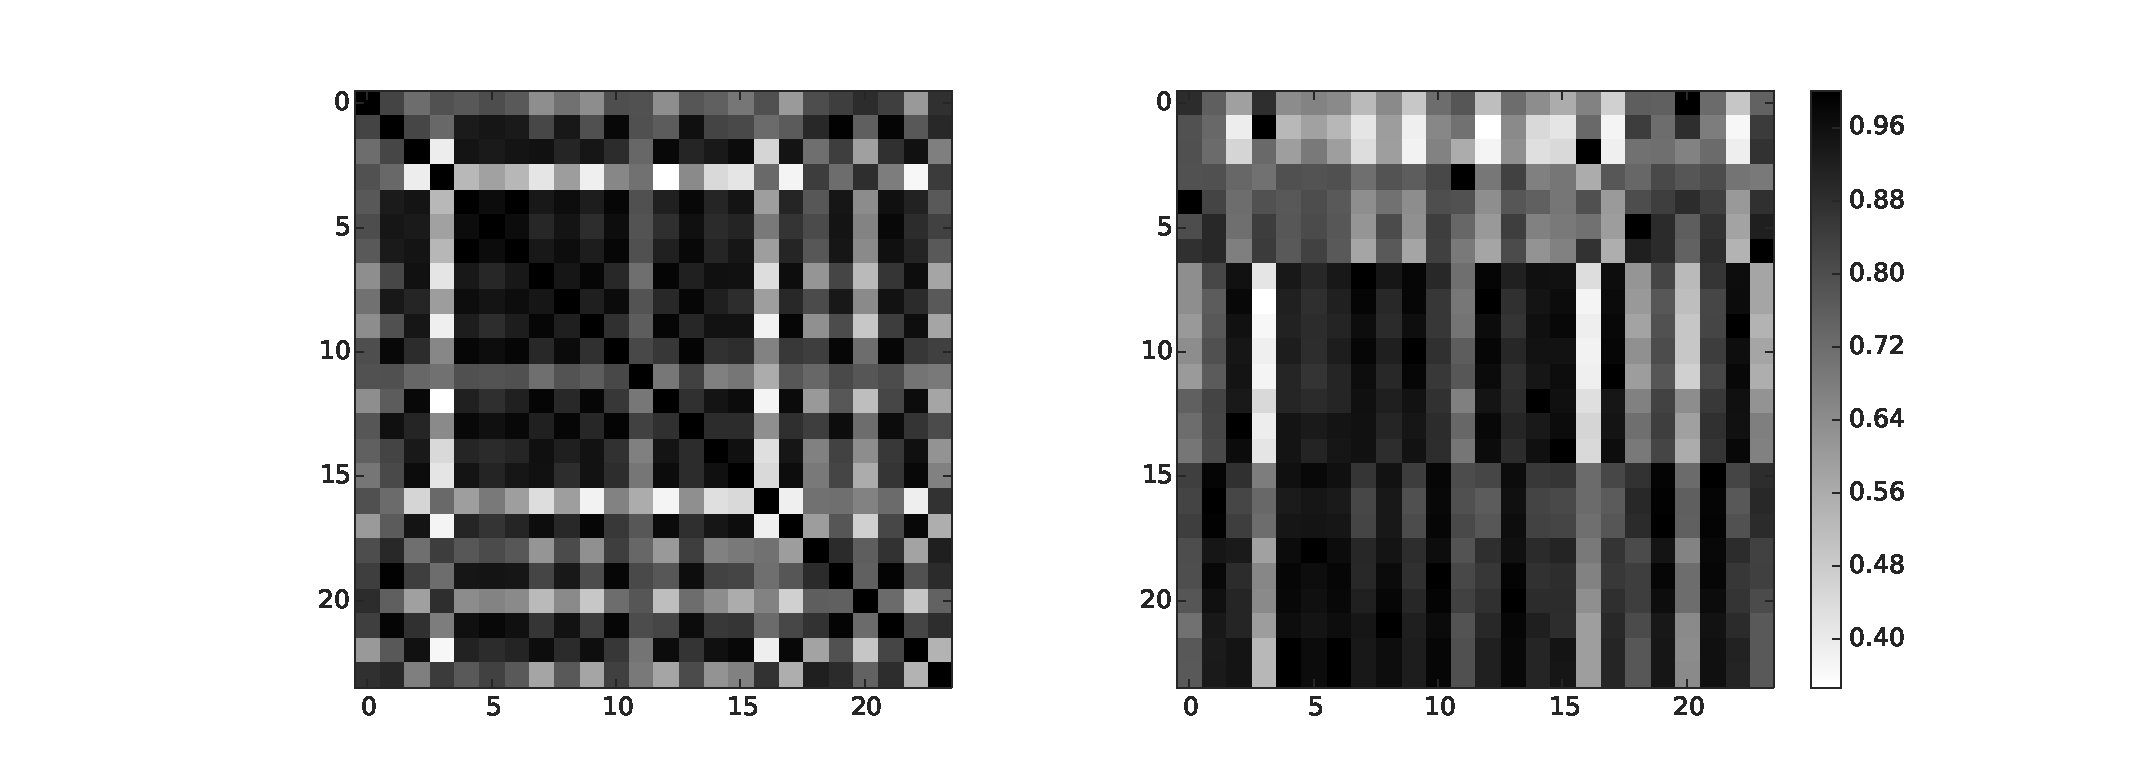
\includegraphics[width=0.7\textwidth]{tex/ASME-journal/results/signals/correlation.eps}
%                 \caption{24x24 Correlation matrix of signals used for each muscle before and after reordering using hierarchical clustering. }
% 				\label{fig:correlation}
%         \end{subfigure}\\
%         \begin{subfigure}[b]{\columnwidth}
%         		\centering
%                 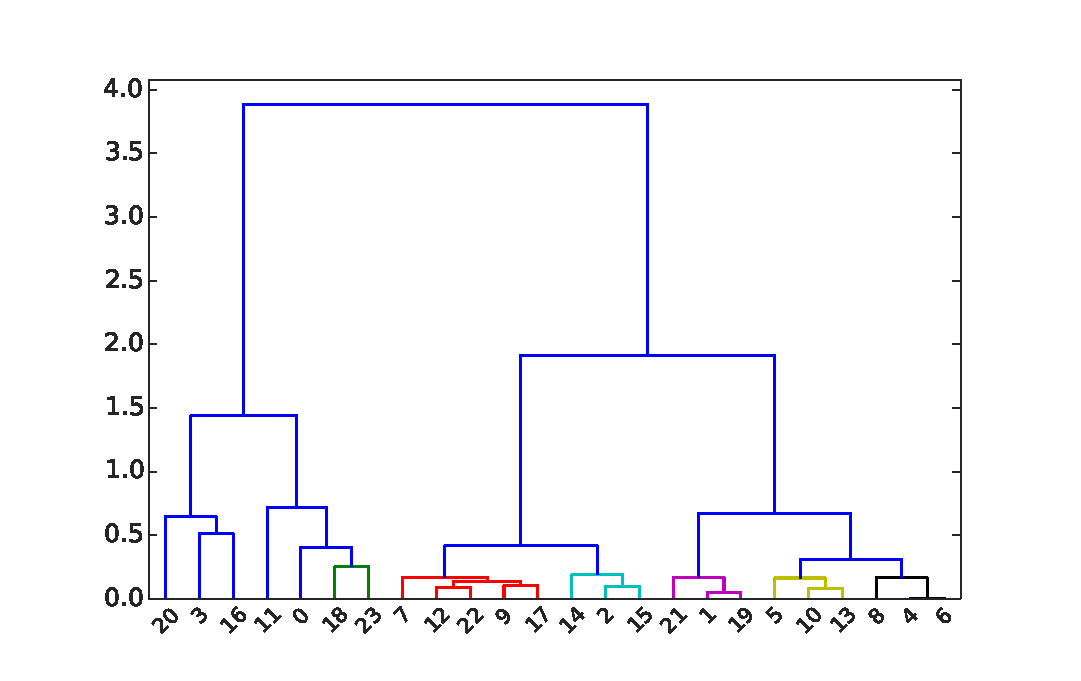
\includegraphics[width=0.7\textwidth]{tex/ASME-journal/results/signals/clustering.eps}
%                 \caption{Result of Hierarchical clustering to cluster and reorder similar signals}
% 				\label{fig:clustering}
%         \end{subfigure}\\
%         \begin{subfigure}[b]{\columnwidth}
%         		\centering
%                 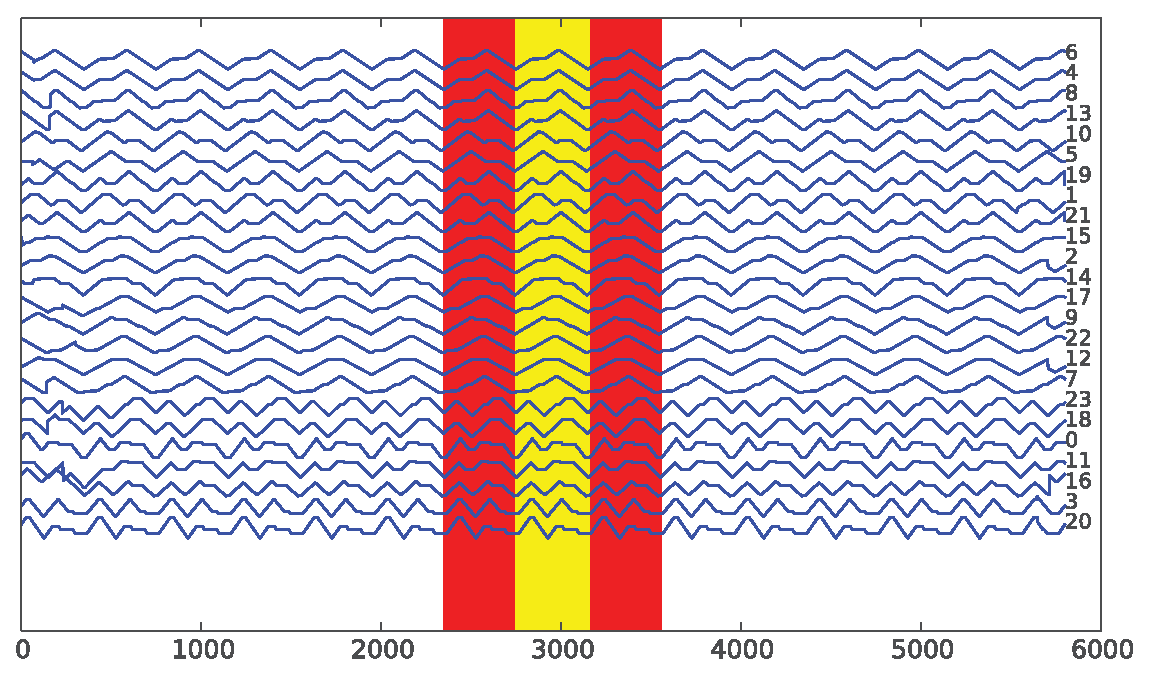
\includegraphics[width=0.7\textwidth]{tex/ASME-journal/results/signals/aligned2.eps}
%                 \caption{The signals for the MUSCLES when they are shifted according to the highest correlation and reordered according to the hierarchical clustering. }
% 				\label{fig:aligned2}
%         \end{subfigure}
%         \caption{The process of analyzing the signals used for the muscles. The signals are shifted and reordered to show similarities. Subfigure (d) shows that groups of signals have similar patterns.}
%         \label{fig:correlationAll}
% \end{figure}

% Next, WE analyze the signals further by looking at their shapes and correlation between them. The top half of the Figure \ref{fig:aligned1} shows all 24 signals when they are normalized between 0 and 1. The purpose of this experiment is to show similarities of signals and different types of signals learned at the end of coevolution. First, WE look at the correlation between signals. For each signal, red-yellow-red area highlights the interval that maximizes correlation with other signals. At this ordering, it is hard to see similarities between signals. In Figure \ref{fig:aligned2}, WE shift the signals so that their selected intervals match, then WE use hierarchical clustering (Figure \ref{fig:clustering}) to group the signals according to the similarity metric. 

% After reordering the signals, Figure \ref{fig:aligned2} shows that half of the signals have one peak high and one low, but the other half have 2 signals that are more complex with 2 peak points. This result gives us multiple conclusions. First, the learning algorithm makes use of the complexity provided. Although a subset of the signals is simple, but another subset has more complex signals with  multiple peak points that can only be generated with complexity coefficients that are higher than 3. The subsets of the signals that are similar can be regenerated using different parameters but the same formula. Let's consider a normalized signal as $f(x)$. The formula $g(x)=A+B*f(x+C)$ can produce similar signals for different values of $A$, $B$ and $C$. Using this idea, all 24 signals can be reproduced using 3 to 4 base functions and different parameters. This gives us a hint about why many papers in literature proposes to use central pattern generators to control tensegrity robots. 

% The last set of results show how critical each muscle is for a given rolling locomotion. WE take the tensegrity robot with the learned policy and disable one of the MUSCLES and observe the effect of such a failure on overall behavior. Figure \ref{fig:disable1} shows that performance depends on which muscle fails. For a significant number of muscles, using the same algorithm still provides rolling behavior with similar performance.  On the other hand some MUSCLES play a critical role for that specific policy.

% \begin{figure}[t]
% \centering
% 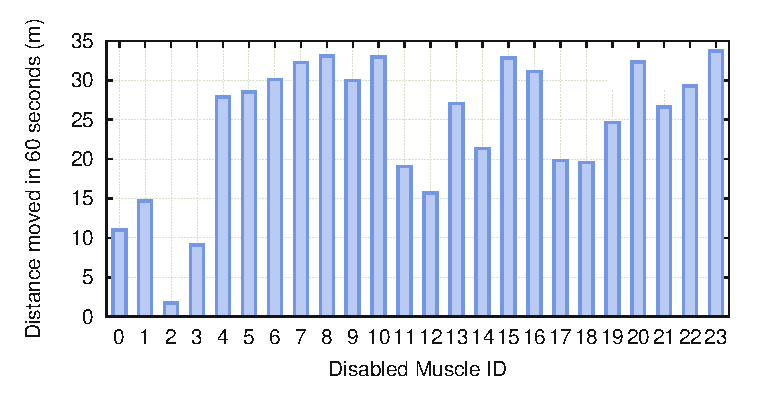
\includegraphics[width=\columnwidth]{tex/ASME-journal/results/testing-disabling1/disabled.eps}
% \caption{The performance of the learned policy, when WE disable one of the muscles. Learned policy is partially robust to failures of some of the muscles. }
% \label{fig:disable1}
% \end{figure}
